\documentclass{article}

\usepackage{tikz}
\usetikzlibrary{bayesnet}

\pagestyle{empty}

\begin{document}
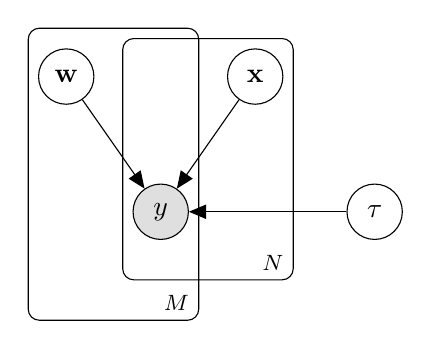
\begin{tikzpicture}

  % Define nodes
  \node[obs]                             (y) {$y$};
  \node[latent, above=of y, xshift=-1.2cm] (w) {$\mathbf{w}$};
  \node[latent, above=of y, xshift=1.2cm]  (x) {$\mathbf{x}$};
  \node[latent, right=2cm of y]              (t) {$\tau$};

  % Connect the nodes
  \edge {x,w,t} {y} ; %

  % Plates
  \plate {yx} {(x)(y)} {$N$} ;
  \plate {} {(w)(y)(yx.north west)(yx.south west)} {$M$} ;

\end{tikzpicture}
\end{document}

%%% Local Variables: 
%%% mode: tex-pdf
%%% TeX-master: t
%%% End: 
